\section{Experiments}
\label{sec:experiments}
In the comparison tables, pale green identifies the proposed method or its stated curvature-learning component. Bold marks the best displayed value within each comparison, including ties at the shown precision; it does not denote statistical significance.
\paragraph{Historical evidence and protocol audit.}
The historical KG tables below use a single-seed exploratory protocol. Inspection of the original KG source shows that both labels B3 and B4 use Euclidean Adam on origin-tangent parameters; B3 in these KG tables is therefore a fixed-curvature Adam model, not the fixed-curvature Riemannian momentum baseline used for synthetic experiments. KG evaluation is unfiltered, tail-only, and uses changing sampled triples. The quoted improvements are valid only for that historical protocol and must not be compared to standard filtered benchmark scores. The revision suite uses actual manifold states and filtered head-and-tail ranking, and its results are kept separate.\par


All experiments use seed 42, as required by the project protocol. We therefore do not report across-seed means, standard deviations, or confidence intervals. For the historical KG results, MRR is evaluated every 25 epochs and is visibly noisy; conclusions use last-5 or last-10 evaluation moving averages rather than single endpoint MRR values. The synthetic experiments run for 1000 or 2000 epochs depending on the sweep, and the KG WN18RR main comparison runs for 2000 epochs. In historical synthetic experiments B3 denotes fixed-curvature momentum, B4 denotes learnable-curvature RSGD without momentum, and B5 additionally uses momentum and normalized steps. Therefore B5 versus B4 is a combined-mechanism comparison, not an isolated test of cross-curvature transport; B5 versus A5 with identical momentum and normalization isolates transport. KG labels follow the distinct Adam protocol described above. The full historical CSV tables used here are copied into \texttt{paper/tables/}.

\subsection{Main results on knowledge graphs}

Table~\ref{tab:kg-main} presents the main KG evidence. On WN18RR, the robust signal is not single-point MRR. B4 improves Hits@10 from 0.3510 to 0.3652 over the last-5 window, a relative gain of $+4.1\%$, and reduces loss from 2.1274 to 2.0680, a relative reduction of $-2.8\%$. MRR is positive but window-sensitive: last-5 MRR changes from 0.1332 to 0.1345 ($+1.0\%$), while last-10 MRR changes from 0.1326 to 0.1357 ($+2.3\%$). On FB15k-237, the metric profile changes: B4 improves MRR from 0.1853 to 0.1893 ($+2.2\%$) and Hits@1 by $+3.1\%$, while Hits@10 is nearly flat at $+0.1\%$ and loss improves by only $-0.9\%$. The honest cross-dataset claim is therefore that grouped learnable curvature improves ranking MRR on both KG datasets, while the affected Hits metric depends on relation structure.

\begin{table}[t]
\centering
\caption{\textbf{Historical WN18RR ranking and fitting.} B3 and B4 use the historical Euclidean-Adam protocol; B4 learns curvature and is shaded. Best values within each window are bold, including B3 on Hits@1. These unfiltered tail-only scores are separate from the new filtered protocol.}
\label{tab:kg-main}
\footnotesize\setlength{\tabcolsep}{4.2pt}\renewcommand{\arraystretch}{1.12}
\begin{adjustbox}{max width=\linewidth}
\begin{tabular}{lrrrr}
\toprule
Method & MRR $\uparrow$ & Hits@1 $\uparrow$ & Hits@10 $\uparrow$ & Loss $\downarrow$ \\
\midrule
\multicolumn{5}{l}{\textit{WN18RR, last 5 evaluations}} \\
B3 & 0.1332 & \textbf{0.0282} & 0.3510 & 2.1274 \\
\rowcolor{oursbg}
B4 & \textbf{0.1345} & 0.0270 & \textbf{0.3652} & \textbf{2.0680} \\
\multicolumn{5}{l}{\textit{WN18RR, last 10 evaluations}} \\
B3 & 0.1326 & \textbf{0.0280} & 0.3491 & 2.1274 \\
\rowcolor{oursbg}
B4 & \textbf{0.1357} & 0.0268 & \textbf{0.3685} & \textbf{2.0678} \\
\bottomrule
\end{tabular}
\end{adjustbox}
\end{table}


Figure~\ref{fig:kg-loss} and Table~\ref{tab:kg-checkpoints} explain why the WN18RR conclusion is phrased this way. B4's loss advantage appears around epoch 300 and persists through epoch 1999, while $\Kstd$ grows from 0.077 at epoch 100 to 0.295 at epoch 1999. The endpoint MRR itself can swing strongly between evaluations, so MRR is treated as supporting evidence rather than the headline metric. This is also why the main claim does not say that Hits@10 consistently improves across KG datasets: FB15k-237 does not support that statement.

\begin{figure}[t]
\centering
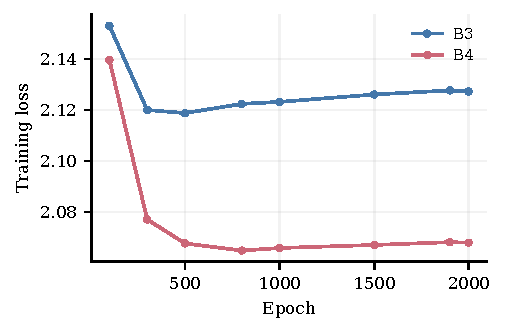
\includegraphics[width=\linewidth]{figures/fig_loss_historical_kg}
\caption{Historical WN18RR training loss at every retained checkpoint. B3 uses fixed curvature and B4 learns curvature. Ranking and curvature checkpoints appear in Table~\ref{tab:kg-checkpoints}.}
\label{fig:kg-loss}
\end{figure}

\subsection{Curvature differentiates by semantic and structural role}

The strongest mechanism evidence is curvature differentiation. On WN18RR, B4 learns $K=2.000$ for \emph{derivationally related form}, $K=1.417$ for \emph{hypernym}, and $K=1.008$ for \emph{similar to}. The spread from 2.000 to 1.008 reflects taxonomic and part-whole relations taking higher curvature, while flatter symmetric relations remain close to the fixed baseline. FB15k-237 has much weaker hierarchy: its $\Kstd=0.071$ is about one quarter of WN18RR's $\Kstd=0.30$, and the high-curvature top relations are award, film, and genre relations rather than clean taxonomic edges. This contrast supports the mechanism claim that learned curvature scales with hierarchical or relational-complexity strength.

Synthetic heterogeneity gives a controlled version of the same effect. In the branching sweep with branchings $[2,8,32,128]$, B4 learns $K=[0.768,0.939,1.011,1.028]$ and B5 learns $K=[0.772,0.945,1.016,1.033]$. The final distortion improves from 0.22870 for B3 to 0.22390 for B4 and 0.22360 for B5. These are modest gains, but the monotone curvature ordering and $\Kstd=0.103$ show that curvature is responding to structural heterogeneity rather than drifting randomly.

\begin{table*}[t]
\centering
\caption{\textbf{Branching heterogeneity.} The four groups have branching rates $[2,8,32,128]$. Historical final distortion/loss and all learned group curvatures are reported.}
\label{tab:heterogeneity}
\footnotesize\setlength{\tabcolsep}{4.2pt}\renewcommand{\arraystretch}{1.12}
\begin{adjustbox}{max width=\linewidth}
\begin{tabular}{lrrrrrr}
\toprule
Method & Distortion $\downarrow$ & Loss $\downarrow$ & $K_1$ & $K_2$ & $K_3$ & $K_4$ \\
\midrule
B3 & 0.22870 & 0.11706 & 1.0000 & 1.0000 & 1.0000 & 1.0000 \\
B4 & 0.22390 & 0.11569 & 0.7681 & 0.9389 & 1.0109 & 1.0280 \\
\rowcolor{oursbg}
B5 & \textbf{0.22360} & \textbf{0.11559} & 0.7719 & 0.9452 & 1.0164 & 1.0328 \\
\bottomrule
\end{tabular}
\end{adjustbox}
\end{table*}


\subsection{Synthetic convergence: speed rather than final-value dominance}

The synthetic 2000-epoch convergence experiment isolates G8. Table~\ref{tab:g8} shows that B4 and B5 reach lower distortion earlier than B3, with the largest relative advantage at epoch 800: B4 is at 0.25160 versus B3 at 0.25674 ($-2.01\%$), and B5 is at 0.25113 ($-2.19\%$). By epoch 1999, B3 has almost closed the gap: B4 is 0.22569 versus B3 0.22641 ($-0.32\%$), and B5 is 0.22555 ($-0.38\%$). We therefore do not claim synthetic final-value superiority. The supported claim is faster convergence in the middle of training.



\begin{table*}[t]
\centering
\caption{\textbf{Complete recorded G8 distortion checkpoints.} Distortion and its relative change use the same recorded checkpoints for every method. Negative changes favor the corresponding learned-curvature method.}
\label{tab:g8}
\footnotesize\setlength{\tabcolsep}{4.2pt}\renewcommand{\arraystretch}{1.12}
\begin{adjustbox}{max width=\linewidth}
\begin{tabular}{lrrrrr}
\toprule
Epoch & B3 & B4 & B5 & $\Delta$ B4/B3 & $\Delta$ B5/B3 \\
\midrule
50 & 0.88271 & \textbf{0.85864} & \cellcolor{oursbg}0.88271 & -2.73\% & -0.0\% \\
100 & 0.73688 & \textbf{0.71515} & \cellcolor{oursbg}0.73632 & -2.95\% & -0.08\% \\
200 & 0.50881 & \textbf{0.49890} & \cellcolor{oursbg}0.50477 & -1.95\% & -0.79\% \\
400 & 0.33409 & 0.32862 & \cellcolor{oursbg}\textbf{0.32798} & -1.64\% & -1.83\% \\
600 & 0.28018 & 0.27487 & \cellcolor{oursbg}\textbf{0.27425} & -1.9\% & -2.12\% \\
800 & 0.25674 & 0.25160 & \cellcolor{oursbg}\textbf{0.25113} & -2.01\% & -2.19\% \\
1000 & 0.24435 & 0.23980 & \cellcolor{oursbg}\textbf{0.23943} & -1.86\% & -2.01\% \\
1200 & 0.23705 & 0.23344 & \cellcolor{oursbg}\textbf{0.23316} & -1.52\% & -1.64\% \\
1500 & 0.23097 & 0.22869 & \cellcolor{oursbg}\textbf{0.22849} & -0.99\% & -1.07\% \\
1999 & 0.22641 & 0.22569 & \cellcolor{oursbg}\textbf{0.22555} & -0.32\% & -0.38\% \\
\bottomrule
\end{tabular}
\end{adjustbox}
\end{table*}


% WWW_REFERENCE_STYLE
\paragraph{Complete product-factor grid.}
The revision also completes all 288 runs in the product-factor tree grid: four tree constructions, three node counts, four total dimensions, and six methods, each trained for 2000 updates with seed 42. B5 has numerically lower final fixed-pair distortion than fixed-curvature momentum B3 in 48/48 configurations, with relative reductions from $0.0022\%$ to $0.7910\%$ (Table~\ref{tab:revision-synthetic-complete}). This is a small, consistent descriptive contrast within the manifold implementation. B5 beats the Euclidean control in 0/48 configurations; its relative distortion difference from A5 never exceeds $0.0059\%$. Thus this grid supports a narrow combined curvature-and-normalization comparison with B3, not overall superiority or a separately established transport benefit. These are fixed-step, single-seed reconstruction measurements without held-out pair selection or an equal-budget hyperparameter search. All 48 configurations and all six methods appear in Appendix~\ref{app:complete-product-grid}; the grid is distinct from the independent-tree drift experiments.

% WWW_REFERENCE_STYLE
\begin{table*}[t]
\centering
\caption{\textbf{Complete product-factor grid: the B5--B3 contrast.} Each tree construction includes all $n\in\{1000,5000,10000\}$ and $d\in\{2,5,10,20\}$. Reduction is $100(1-D_{\rm B5}/D_{\rm B3})$, in percent, from unrounded final fixed-pair distortion. Counts use strict numerical comparisons, not significance tests. Every configuration is retained. The final column shows the broader Euclidean comparison.}
\label{tab:revision-synthetic-complete}
\footnotesize\setlength{\tabcolsep}{4.2pt}\renewcommand{\arraystretch}{1.12}
\begin{tabular}{lrrrr}
\toprule
Tree & B5 $<$ B3 & Reduction range (\%) & Median reduction (\%) & B5 $<$ E \\
\midrule
Binary & \cellcolor{oursbg}12/12 & 0.0022--0.3247 & 0.0118 & 0/12 \\
4-ary & \cellcolor{oursbg}12/12 & 0.0159--0.7910 & 0.0794 & 0/12 \\
8-ary & \cellcolor{oursbg}12/12 & 0.0509--0.3624 & 0.2308 & 0/12 \\
Variable & \cellcolor{oursbg}12/12 & 0.0101--0.6402 & 0.0472 & 0/12 \\
\bottomrule
\end{tabular}
\end{table*}


\subsection{Expanded paired comparisons and long-horizon mechanism tests}
The completed mechanism matrix contains 60 initial 2000-update runs and 48 matched-initialization controls. Four independent trees contain 250 nodes each, with three-dimensional embeddings per group. We use branchings $[2,4,8,16]$ for a stationary control and smooth distance-scaling endpoints $2$, $5$, and $8$, plus an abrupt $8\times$ scaling at the midpoint; a separate stationary heterogeneity case uses branchings $[2,8,32,128]$. For smooth drift, group $g\in\{1,2,3,4\}$ has target metric $D_{g,t}=D_g[1+(s_{\rm end}-1)g\,t/(4(T-1))]$. Positive scalar rescaling preserves the tree metric. A fixed seed partitions the unordered pairs in each tree into 80\% training, 10\% validation, and 10\% test pairs, identically for every method. The training objective sums group mean squared relative-distance errors. Test distortion is evaluated only at the final update; the mean validation distortion over all updates measures tracking performance.

The common settings are $\eta=100$, $\rho=0.01$, $\beta=0.98$, $\gamma=1$, $K\in[0.001,5]$, a $0.01$ log-curvature cap, a $0.25$ normalized geodesic trust cap, and $\sqrt K r\le4$. All optimization uses FP32; a separate FP64 diagnostic measures the constraint residual of the stored points. B5 versus A5 isolates the cross-curvature momentum map. B3 tests fixed curvature, B35 adds normalized steps at fixed curvature, B4 removes momentum, and the shared-curvature variant tests group adaptation. B35 additionally receives $K\in\{0.03,0.1,0.3,1,3\}$: the best fixed value is selected by final validation distortion only after all five runs finish. Initial validation results revealed substantial sensitivity to this choice, so B5 and A5 receive the same five initial values in a matched search amendment. This exploratory extension retains the original runs and makes no sealed-test or confirmatory claim. The selected comparison requires all 15 runs per case, a condition now met for all six cases. B5 versus A5 at the same selected initialization remains a separate transport contrast. The experiment uses the total curvature derivative through the point homothety; it is separate from the historical partial-derivative drift diagnostic and from the product-factor synthetic benchmark.

% WWW_REFERENCE_STYLE
\begin{table}[t]
\centering
\footnotesize\setlength{\tabcolsep}{4.2pt}\renewcommand{\arraystretch}{1.12}
\caption{Selected synthetic conditions with at least 0.5\% lower test distortion than validation-selected fixed curvature. Each method receives the same five initializations and 2000 updates. This is an outcome-selected display from six cases; all cases, including ties and negative results, appear in Appendix~\ref{app:extended-audit}. Different drift conditions are not different task families.}
\label{tab:revision-mechanism-focus}
\begin{adjustbox}{max width=\linewidth}
\begin{tabular}{lrrrr}
\toprule
Condition & Best fixed & B5 & Best A5 & Reduction \\
\midrule
smooth2 & 0.1823 & \cellcolor{oursbg}\textbf{0.1762} & 0.1763 & 3.31\% \\
smooth8 & 0.2757 & \cellcolor{oursbg}\textbf{0.2619} & 0.2624 & 5.02\% \\
static & 0.2011 & \cellcolor{oursbg}0.1952 & \textbf{0.1951} & 2.94\% \\
\bottomrule
\end{tabular}
\end{adjustbox}
\end{table}


All 108 mechanism runs have now completed. With the same five-initialization budget and selection by final validation distortion, B5 reduces held-out distortion relative to normalized fixed-curvature momentum B35 by $2.94\%$ in the stationary control, $3.31\%$ under $2\times$ smooth drift, and $5.02\%$ under $8\times$ smooth drift. Table~\ref{tab:revision-mechanism-focus} focuses on these stronger decreases. This is an explicitly outcome-selected presentation from six cases; the full comparison, including the nearly tied $5\times$ case and the negative abrupt-drift case, is retained in Appendix~\ref{app:extended-audit}. The smaller heterogeneous-case decrease is quantified separately in Table~\ref{tab:positive-narrow-contrasts}; the $0.5\%$ display rule for the focus table is unchanged. These are different conditions in one synthetic family. A5 remains close to B5, so the selected scores support curvature adaptation rather than an isolated transport-performance claim.

At the common initialization $K_0=1$, the completed $2\times$, $5\times$, and $8\times$ smooth-drift runs give final held-out distortions $0.32953$, $0.43471$, and $0.48132$ for B5, versus $0.33276$, $0.62251$, and $0.74110$ for fixed-curvature B3. The relative reductions are $0.97\%$, $30.17\%$, and $35.05\%$. Figure~\ref{fig:loss-drift} shows the complete training-loss trajectories; Table~\ref{tab:drift-states} gives validation distortion and learned curvature checkpoints. The advantage remains at the complete 2000-update endpoint relative to the \emph{same-initialization, fixed-$K=1$} momentum control. Because the common safety constraint is $\sqrt K r\le4$, changing curvature also changes the admissible physical-distance range. The experiment therefore combines online scale adaptation with feasible-set capacity; it is not a pure optimizer comparison on a fixed hypothesis class. A5 is within $0.02\%$ of B5 in final distortion in all three cases, so these trained-model results do not isolate a transport benefit. Moreover, low fixed-curvature settings perform substantially better than $K=1$ in the validation sweep. The larger common-initialization percentages are therefore distinguished from the smaller gains against the validation-selected fixed-curvature control reported above.

\begin{figure*}[t]
\centering
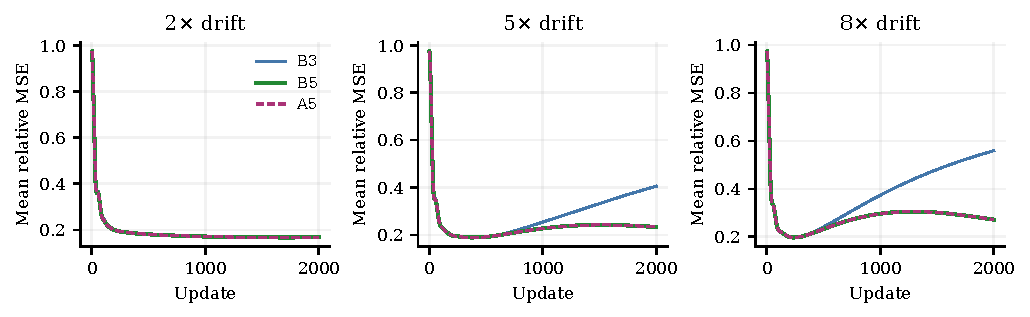
\includegraphics[width=\linewidth]{figures/fig_loss_smooth_drift}
\caption{Complete training-loss trajectories under smooth distance drift: $2\times$, $5\times$, and $8\times$ from left to right. All methods share $K_0=1$ and run for 2000 updates. Each panel shows the logged mean squared relative-distance loss; validation distortion and B5 curvature states are tabulated in Table~\ref{tab:drift-states}. These curves are separate from the validation-selected initialization comparison.}
\label{fig:loss-drift}
\end{figure*}

For completeness, the other three common-$K_0=1$ conditions also favor B5 over B3 in final held-out distortion: $0.272665$ versus $0.273396$ in the stationary case ($0.27\%$ lower), $0.246959$ versus $0.250953$ under heterogeneous branching ($1.59\%$ lower), and $0.617550$ versus $0.741727$ after abrupt scaling ($16.74\%$ lower). Thus all six common-initialization contrasts against B3 are positive. This statement concerns the specified initialization: after the matched five-value validation search, the abrupt case instead gives B5 distortion $0.165479$ versus B35 $0.163686$, a $1.09\%$ increase. The distinction between a fixed initialization and a selected fixed-curvature control is preserved throughout.


\subsection{Direct checks of the geometric mechanisms}
\label{sec:revision-operator-checks}
Tables~\ref{tab:sensitivity} and~\ref{tab:operator-transport} test two exact geometric predictions on compute environment. First, we perturb momentum transversely at the origin for $K\in\{0.01,0.1,1,10,100\}$, with nominal $\eta=\gamma=1$. The measured amplification follows the exact Jacobi--normalization differential in Theorem~\ref{thm:sharp-normalized-exp}; the maximum relative discrepancy in the FP64 reference check for $\sqrt K\|m\|\ge0.1$ is $5.1\times10^{-8}$. Curvature-scaled inputs share the same exact amplification values. The control here is the uncapped exponential map: this operator experiment deliberately omits the extra trust cap used in the training implementation, and it does not measure a training-speed advantage.

Second, we prescribe $K_t=s^{-2t/2000}$ for $s\in\{2,5,8\}$ and apply a constant unit canonical gradient with $\beta=0.98$. With zero initial momentum and no position motion, the exact canonical recurrence is $p_t=1-\beta^{t+1}$. Point-and-momentum transport preserves this recurrence to a maximum FP32 absolute error of $3.2\times10^{-6}$ over all three trajectories. Mapping only the point produces final canonical errors of $0.0170$, $0.0387$, and $0.0494$, respectively. Thus this controlled experiment isolates accumulated momentum-scale mismatch. Curvature is prescribed rather than learned here, so the result establishes a geometric consistency advantage, not a downstream accuracy or generalization improvement.

\begin{table}[t]
\centering
\caption{\textbf{Measured sensitivity check.} FP64 transverse finite perturbations use all five $K\in\{0.01,0.1,1,10,100\}$. Exact gains are listed; the final column is the largest measured relative discrepancy across these curvatures and both operators. No trust cap is used in this operator check.}
\label{tab:sensitivity}
\footnotesize\setlength{\tabcolsep}{4.2pt}\renewcommand{\arraystretch}{1.12}
\begin{adjustbox}{max width=\linewidth}
\begin{tabular}{lrrr}
\toprule
\makecell{Scaled\\momentum} & \makecell{Uncapped\\gain} & \makecell{Normalized\\gain} & \makecell{Max. rel.\\error $\downarrow$} \\
\midrule
0.1 & 1.00167 & 0.910344 & 4.44e-10 \\
1 & 1.1752 & 0.521095 & 1.56e-11 \\
10 & 1101.32 & 0.103959 & 5.05e-08 \\
\bottomrule
\end{tabular}
\end{adjustbox}
\end{table}

\begin{table*}[t]
\centering
\caption{\textbf{Cross-curvature state consistency.} Curvature drift is prescribed, gradients are canonical constants, and the position does not move. This isolates optimizer-state consistency; it is not a downstream accuracy comparison.}
\label{tab:operator-transport}
\footnotesize\setlength{\tabcolsep}{4.2pt}\renewcommand{\arraystretch}{1.12}
\begin{adjustbox}{max width=\linewidth}
\begin{tabular}{lrrr}
\toprule
State mapping & $2\times$ drift & $5\times$ drift & $8\times$ drift \\
\midrule
\multicolumn{4}{l}{\textit{FP32, maximum absolute canonical momentum error over 2000 updates}} \\
Point only & 1.70e-02 & 3.87e-02 & 4.94e-02 \\
\rowcolor{oursbg}
Point + momentum & \textbf{3.13e-06} & \textbf{1.03e-06} & \textbf{1.84e-06} \\
\multicolumn{4}{l}{\textit{FP64, maximum absolute canonical momentum error over 2000 updates}} \\
Point only & 1.70e-02 & 3.87e-02 & 4.94e-02 \\
\rowcolor{oursbg}
Point + momentum & \textbf{2.55e-15} & \textbf{6.22e-15} & \textbf{4.22e-15} \\
\bottomrule
\end{tabular}
\end{adjustbox}
\end{table*}


\paragraph{Preliminary smooth-drift transport evidence.}
The original project also contains 400-epoch synthetic drift diagnostics, below the proposal's formal training-length requirement. They compare B5 with A5 while smoothly scaling target distances. Distortion AUC changes from 0.4460 to 0.4431 for a $2\times$ drift, from 0.5220 to 0.5105 for $5\times$, and from 0.6191 to 0.5968 for $8\times$. The corresponding relative reductions are 0.64\%, 2.19\%, and 3.60\%. The original report also records a negative abrupt-shift comparison and an unsuccessful Rotated MNIST curvature-load diagnostic. These observations motivate transport checks but do not establish necessary-and-sufficient conditions, a real-data transport win, or another completed task family. Their source is retained in \texttt{experiments/G4\_MECHANISM\_EVIDENCE.md}.

\subsection{Additional positive contrasts with explicit controls}
\label{sec:additional-positive}
\paragraph{Node classification at the fixed endpoint.}
B5 improves final test accuracy over B3 in five of the 12 completed dataset--encoder pairs: ogbn-arxiv/GAT, ogbn-arxiv/GraphSAGE, Citeseer/GraphSAGE, Cora/GCN, and PubMed/GraphSAGE. Table~\ref{tab:positive-graph-contrasts} reports every such positive final contrast, with gains of $0.076$--$0.278$ percentage points, together with the Euclidean and A5 controls. This is an explicitly outcome-selected presentation of the original final-checkpoint endpoint, not a new selection rule or an additional family-level claim. The Euclidean control remains stronger on both ogbn-arxiv rows and Cora/GCN; A5 ties B5 on the Citeseer, Cora, and PubMed rows. Checkpoint choice also matters: Citeseer/GraphSAGE and PubMed/GraphSAGE have negative B5--B3 differences at the validation-selected checkpoints, which are shown alongside the final differences. All 12 pairs, including ties and negative differences, remain in Appendix~\ref{app:extended-audit}.

% WWW_REFERENCE_STYLE
\begin{table*}[t]
\centering
\caption{\textbf{Positive final-checkpoint graph contrasts against B3.} These five rows are an outcome-selected subset of all 12 completed dataset--encoder pairs; the complete matrix is in Table~\ref{tab:revision-breadth}. Accuracy and differences are in percent and percentage points, respectively. All runs finish 1000 epochs, seed 42. $\Delta_{\rm val}$ separately compares test accuracy at checkpoints selected by validation accuracy; it is not used to choose the displayed endpoint. A dash denotes an unavailable selected-checkpoint record. Bold marks the best displayed final accuracy, including rounded ties, not significance or a family-level win.}
\label{tab:positive-graph-contrasts}
\footnotesize\setlength{\tabcolsep}{6pt}\renewcommand{\arraystretch}{1.12}
\begin{adjustbox}{max width=\linewidth}
\begin{tabular}{lrrrrrr}
\toprule
Dataset / encoder & E & B3 & B5 & A5 & $\Delta_{\rm final}$ & $\Delta_{\rm val}$ \\
\midrule
ogbn-arxiv / GAT & \textbf{68.420} & 62.329 & \cellcolor{oursbg}62.406 & 62.447 & +0.076 & +0.076 \\
ogbn-arxiv / GraphSAGE & \textbf{68.321} & 63.389 & \cellcolor{oursbg}63.667 & 63.502 & +0.278 & +0.276 \\
Citeseer / GraphSAGE & 62.300 & 66.500 & \cellcolor{oursbg}\textbf{66.600} & \textbf{66.600} & +0.100 & -0.300 \\
Cora / GCN & \textbf{77.800} & 77.100 & \cellcolor{oursbg}77.200 & 77.200 & +0.100 & -- \\
PubMed / GraphSAGE & 74.200 & 75.100 & \cellcolor{oursbg}\textbf{75.200} & \textbf{75.200} & +0.100 & -0.100 \\
\bottomrule
\end{tabular}
\end{adjustbox}
\end{table*}


\paragraph{Smaller mechanism and named-control gains.}
Table~\ref{tab:positive-narrow-contrasts} makes four additional positive primary-endpoint contrasts explicit. In the heterogeneous hierarchy, the matched five-initialization validation search gives B5 distortion $0.217679$ versus B35 $0.218234$, a $0.254\%$ reduction; A5 reaches $0.217351$, so this does not isolate a transport gain. On WN18RR translation, grouped B5 improves over shared curvature by $0.000295$ MRR ($0.289\%$ relative), while E and the fixed-curvature controls remain stronger and shared curvature has slightly higher Hits@10. On Rotated MNIST, B5 improves mean accuracy over all five tasks by $0.044$ percentage points relative to B35 and $0.136$ relative to shared curvature. E, B2, and B3 still have higher mean accuracy. These observations identify the exact favorable comparisons without treating individual controls or conditions as independent task families, and without replacing a primary endpoint by a favorable secondary metric.

% WWW_REFERENCE_STYLE
\begin{table*}[t]
\centering
\caption{\textbf{Additional positive contrasts with named controls.} Each row uses its original primary endpoint and full training length. The improvement is relative distortion reduction in the first row, absolute MRR difference in the second, and accuracy difference in percentage points in the last two. These units are not pooled. The A5 column preserves the transport comparison. Bold marks the best displayed score within a row; stronger controls outside these selected contrasts are reported in the full appendix. All are single-seed descriptive comparisons.}
\label{tab:positive-narrow-contrasts}
\footnotesize\setlength{\tabcolsep}{5pt}\renewcommand{\arraystretch}{1.12}
\begin{adjustbox}{max width=\linewidth}
\begin{tabular}{lllrrrr}
\toprule
Case & Control & Primary endpoint & Control score & B5 & A5 & Improvement \\
\midrule
Heterogeneous hierarchy & Selected B35 & Distortion $\downarrow$ & 0.218234 & \cellcolor{oursbg}0.217679 & \textbf{0.217351} & 0.254\% \\
WN18RR / translation & Shared curvature & MRR $\uparrow$ & 0.102000 & \cellcolor{oursbg}\textbf{0.102295} & \textbf{0.102295} & +0.000295 \\
Rotated MNIST / MLP & B35 & Mean accuracy (\%) $\uparrow$ & 43.388 & \cellcolor{oursbg}\textbf{43.432} & 43.378 & +0.044 pp \\
Rotated MNIST / MLP & Shared curvature & Mean accuracy (\%) $\uparrow$ & 43.296 & \cellcolor{oursbg}\textbf{43.432} & 43.378 & +0.136 pp \\
\bottomrule
\end{tabular}
\end{adjustbox}
\end{table*}


\subsection{Prospective real-data task extension}
\label{sec:new-tasks}
To test whether the geometric gains transfer beyond controlled metric drift, we register six additional tasks in three evaluation directions: WordNet mammal and vehicle ancestor completion; Cora and Citeseer held-out-link prediction; and inductive class-relevance retrieval on optical digits and 20 Newsgroups. Taxonomy extends the knowledge-graph family, citation links extend graph learning, and image/text retrieval forms one retrieval family. Neither individual datasets nor synthetic drift settings are counted as additional families. The complete task definitions, data provenance, and unfiltered outcome matrix appear in Appendix~\ref{app:extended-audit}.

Every task receives 30 full-length runs: E, B3, B35, B5, and A5 each receive six configurations and 1000 epochs, with seed 42. The complete grid is fixed before execution. Each method is selected by its final validation primary metric; test evaluation is delayed until all 30 configurations for the task finish. The method uses four two-dimensional factors, and all methods receive the same learned score temperature and bias, so simple score calibration is available to the fixed-curvature controls. The primary endpoints are filtered query MAP for taxonomy, balanced-pair AP for links, and same-class Recall@1 against the training-only gallery for retrieval. All six 30-run blocks and their delayed test evaluations are complete.

\paragraph{Presentation and claim scope.}
For this six-task extension, the main-text display requires B5 to exceed each of E, B3, and B35 by at least 0.5 percentage points in the primary endpoint. This is a disclosed outcome-based presentation rule, not a hypothesis test. A descriptive family-level advantage requires both predeclared tasks in that broad family to meet the rule; all completed task outcomes remain in the appendix. A5 is additionally evaluated at B5's selected hyperparameters to retain a matched transport comparison. Single-seed comparisons cannot establish statistical significance or guarantee benefits on untested tasks. The existing full-data node classification comparisons remain mixed; their complete results are also retained in the appendix.

% WWW_REFERENCE_STYLE
\noindent All six additional tasks have completed their full searches and delayed test evaluations. None meets the stated display criterion; the complete outcomes are retained in the appendix.\par


% WWW_REFERENCE_STYLE
\paragraph{Completed long-horizon classification control.}
The eight-method 20 Newsgroups classification block now completes 1000 epochs per method. Selecting each checkpoint by validation accuracy gives test accuracy $57.674\%$ for B5, $57.820\%$ for B3 and B35, and $61.471\%$ for E. Thus this block does not add a classification-family advantage. Appendix~\ref{app:long-horizon-audit} reports every method, selected epochs, macro-F1, and final endpoints, together with the available full-length WN18RR, MovieLens-1M, and Rotated MNIST comparisons. Partial blocks and secondary-metric increases do not extend the positive family claims.
\paragraph{Additional completed controls.}
For the separate two-layer Transformer on 20 Newsgroups, the completed B5--B3 pair gives validation-selected test accuracy $52.987\%$ versus $54.673\%$ (B5 minus B3: $-1.686$ percentage points). This is one encoder-specific contrast within text classification. All 4 retained Transformer methods are complete; 2 other registered methods were deferred. Table~\ref{tab:revision-transformer-audit} preserves both the selected and final checkpoints. The MovieLens-1M A5 control exactly matches B5 in the recorded final NDCG@20 and Recall@20, so this pair does not isolate a transport-performance advantage. The complete available rows and their primary metrics remain in the appendix.
\paragraph{Completed distance-model comparison.}
All six WN18RR relation-weighted distance configurations complete 2000 epochs. Final filtered MRR is $0.13685$ for B5, $0.14077$ for B3, $0.15722$ for E, and $0.13691$ for A5. This complete block does not add a task-family advantage or an isolated transport gain; Table~\ref{tab:revision-kg-distance-audit} reports all six methods and all ranking endpoints.


\paragraph{Focused completion budget.}
After observing the completed outcomes and execution costs, we reduced the remaining revision workload from 202 to 14 configurations: five ongoing controls, three missing Euclidean controls, and the unopened six-method WN18RR relation-weighted distance block. The last block tests direct metric fitting on a hierarchical graph within the existing KG family; it is a model comparison within that family, not a new task family. This is an exploratory budget amendment, not a prospective confirmatory selection. The original 893-configuration registry remains intact, with all 705 retained configurations now complete and 188 explicitly deferred. All 691 results already completed at the amendment remain in the appendix, irrespective of outcome. Seed, data splits, full training lengths, primary endpoints, and checkpoint-selection rules are unchanged. Appendix~\ref{app:scope-amendment} records the retained comparisons and the interrupted visual run.
